\documentclass[color=usenames,dvipsnames]{beamer}

\mode<presentation> {

\usetheme{Madrid}

\usepackage{tikz}
\usetikzlibrary{shapes.geometric, arrows}

\definecolor{ERC1}{HTML}{C72321}
\definecolor{ERC2}{HTML}{861719}
\definecolor{ERC3}{HTML}{FBD7A9}
\definecolor{ERC4}{HTML}{BA9F7C}
\definecolor{ERC5}{HTML}{7A6952}
\definecolor{ERC6}{HTML}{6E9B9E}
\definecolor{ERC7}{HTML}{0D8085}
\definecolor{ERC8}{HTML}{19484C}
\definecolor{ERC9}{HTML}{F0C320}
\definecolor{ERC10}{HTML}{AF8F19}


\tikzstyle{startstop} = [rectangle, rounded corners, minimum width=3cm, minimum height=1cm,text centered, draw=black, fill=ERC8]
\tikzstyle{io} = [trapezium, trapezium left angle=70, trapezium right angle=110, minimum width=3cm, minimum height=1cm, text centered, draw=black, fill=ERC7]
\tikzstyle{process} = [rectangle, minimum width=3cm, minimum height=1cm, text centered, draw=black, fill=ERC9]
\tikzstyle{decision} = [diamond, minimum width=3cm, minimum height=1cm, text centered, draw=black, fill=ERC10]
\tikzstyle{arrow} = [thick,->,>=stealth]


\setbeamercolor{palette primary}{bg=ERC1,fg=white}
\setbeamercolor{palette secondary}{bg=ERC2,fg=white}
\setbeamercolor{palette tertiary}{bg=ERC3,fg=white}
\setbeamercolor{palette quaternary}{bg=ERC4,fg=white}
\setbeamercolor{structure}{fg=ERC5} % itemize, enumerate, etc
\setbeamercolor{section in toc}{fg=ERC6} % TOC sections

%gets rid of bottom navigation bars
\setbeamertemplate{footline}[frame number]{}

%gets rid of bottom navigation symbols
\setbeamertemplate{navigation symbols}{}

%gets rid of footer
%will override 'frame number' instruction above
%comment out to revert to previous/default definitions
\setbeamertemplate{footline}{}

% Override palette coloring with secondary
%\setbeamercolor{subsection in head/foot}{bg=UBCgrey,fg=white}


%\usecolortheme{lily}
\useoutertheme{infolines}

}


\usepackage{booktabs} 
\usepackage{tikz}


% Thin fonts
\usepackage{cmbright}
\usepackage[T1]{fontenc}

\definecolor{dark_grey}{gray}{0.5}
%\setbeamercolor{normal text}{fg=dark_grey,bg=white}
\setbeamertemplate{navigation symbols}{}

%\setbeamercolor*{palette primary}{fg=gray!100,bg=gray!10}
%\setbeamercolor*{palette quaternary}{fg=gray!100,bg=gray!10}
%\setbeamercolor*{palette secondary}{fg=gray!100,bg=gray!20}
%\setbeamercolor*{palette tertiary}{fg=gray!100,bg=gray!10}
%\setbeamercolor*{navigation symbols}{fg=white,bg=white}
\usefonttheme{default}


\setbeamertemplate{blocks}[rounded][shadow=false]
%\setbeamercolor{block title}{bg=gray!10}
%\setbeamercolor{block body}{fg=gray,bg=gray!10}
%\setbeamercolor{frametitle}{fg=}

\setbeamertemplate{frametitle}[default][center]

\setbeamertemplate{itemize items}[default]
\setbeamertemplate{enumerate items}[default]

\newcommand{\F}{\mathbb{F}}

\setbeamertemplate{title page}[default][colsep=-4bp,rounded=true]

\title[Workshop - Machine Learning]{ Don't believe the hype? A hands-on introduction to machine-learning in Python - Part III.1}
\subtitle{Open Workshops on Computer Based Systems Modelling}

\author{Johannes Schmidt, Johann Baumgartner}
\institute{Institute for Sustainable Economic Development, BOKU, Vienna}
\date{7.05.2019}

\begin{document}

{
\usebackgroundtemplate{
 \begin{picture}(320,315)
 \hspace{6.9cm}
   
\includegraphics[width=0.7\linewidth]{../figures/refuel_logo_with_text.png}
 \end{picture}
 }


\begin{frame}

\maketitle



\end{frame}
}
% Uncomment these lines for an automatically generated outline.
%\begin{frame}{Outline}
%  \tableofcontents
%\end{frame}
%\subsection{Mathematics}

\begin{frame}{Global Power Plant Database: Need for Validation}
\center{
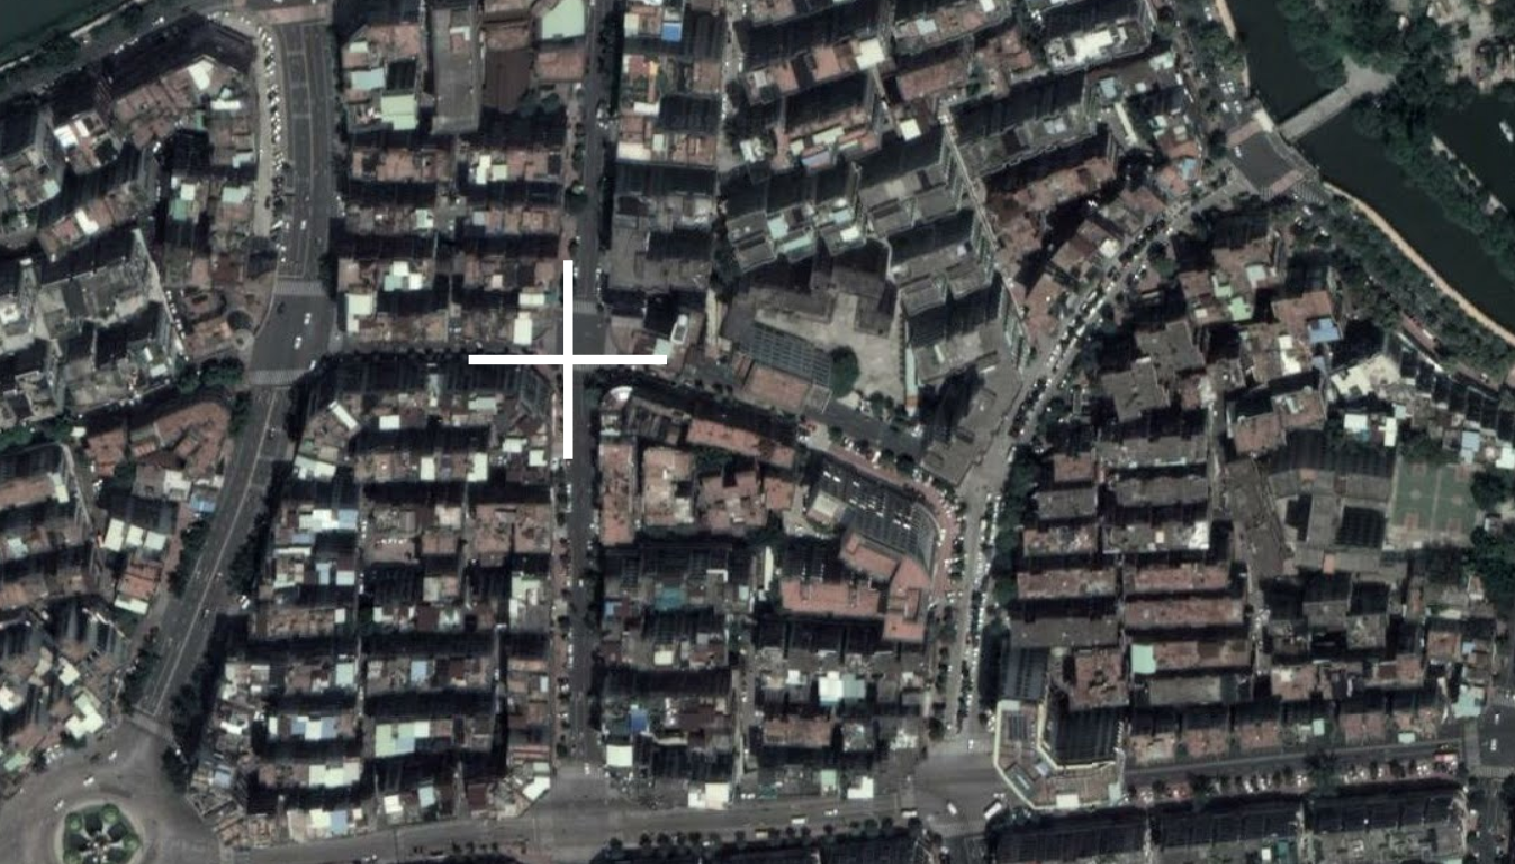
\includegraphics[width=\linewidth]{../figures/wrong_location.png}
}


%Let $X_1, X_2, \ldots, X_n$ be a sequence of independent and identically distributed random variables with $\text{E}[X_i] = \mu$ and $\text{Var}[X_i] = \sigma^2 < \infty$, and let
%$$S_n = \frac{X_1 + X_2 + \cdots + X_n}{n}
%      = \frac{1}{n}\sum_{i}^{n} X_i$$
%denote their mean. Then as $n$ approaches infinity, the random variables $\sqrt{n}(S_n - \mu)$ converge in distribution to a normal $\mathcal{N}(0, \sigma^2)$.

\end{frame}


\begin{frame}

\frametitle{Satellite data for validation}


\framesubtitle{Sentinel-2 (10 meter resolution), free}
	\center{
	
\includegraphics[width=\linewidth]{../figures/sentinel-2.png}
}

\end{frame}

\begin{frame}
\frametitle{Satellite data for validation }
\framesubtitle{WorldView-4, Quickbird (0.31-0.65 meter resolution) used by e.g. Google Maps}

\center{
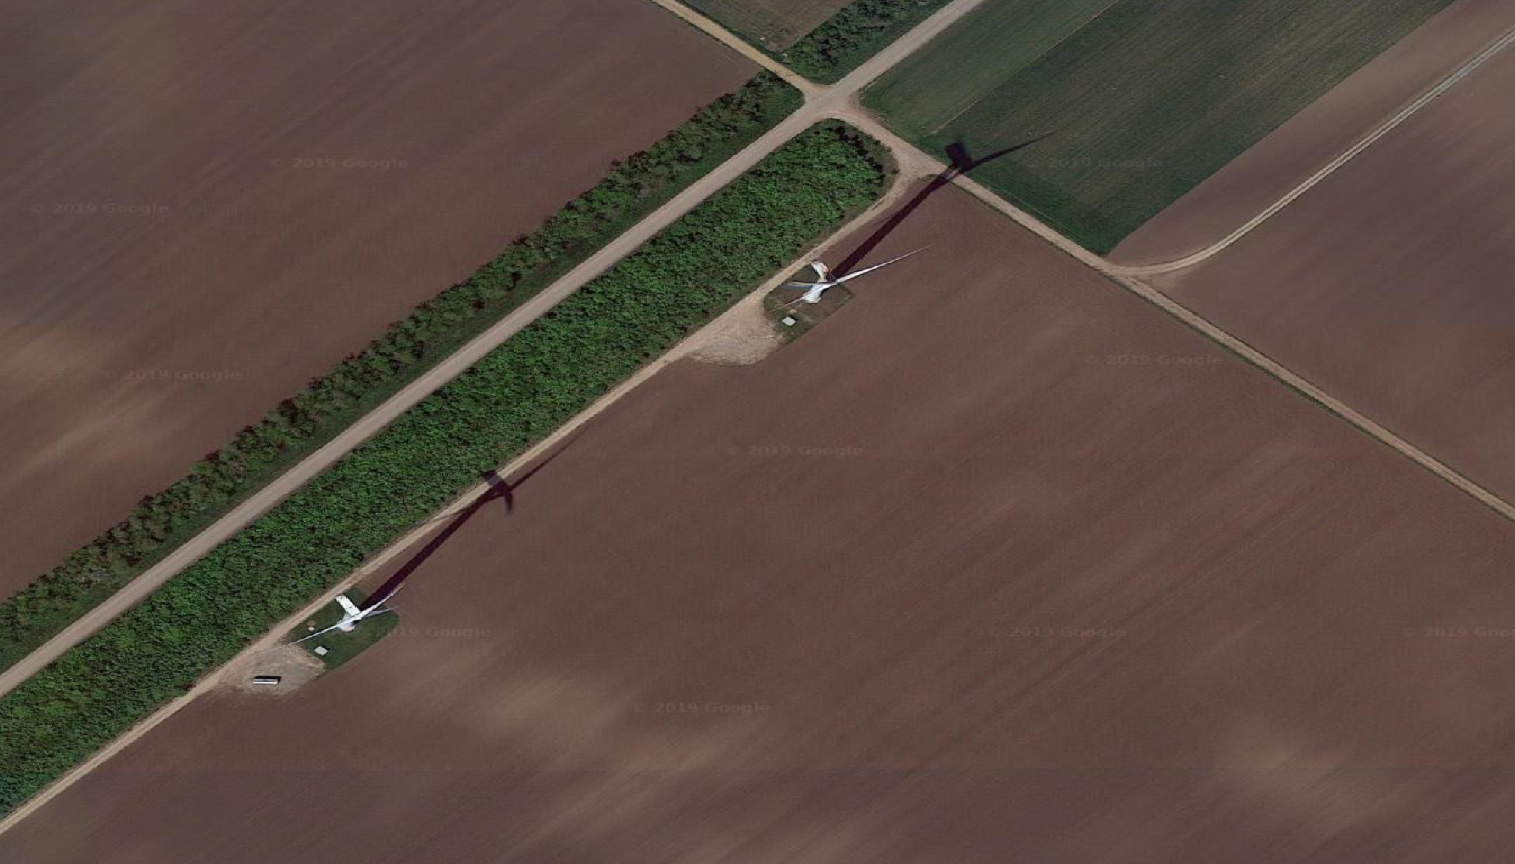
\includegraphics[width=\linewidth]{../figures/googlemaps.png}
}

\end{frame}

\begin{frame}
\frametitle{Approach}

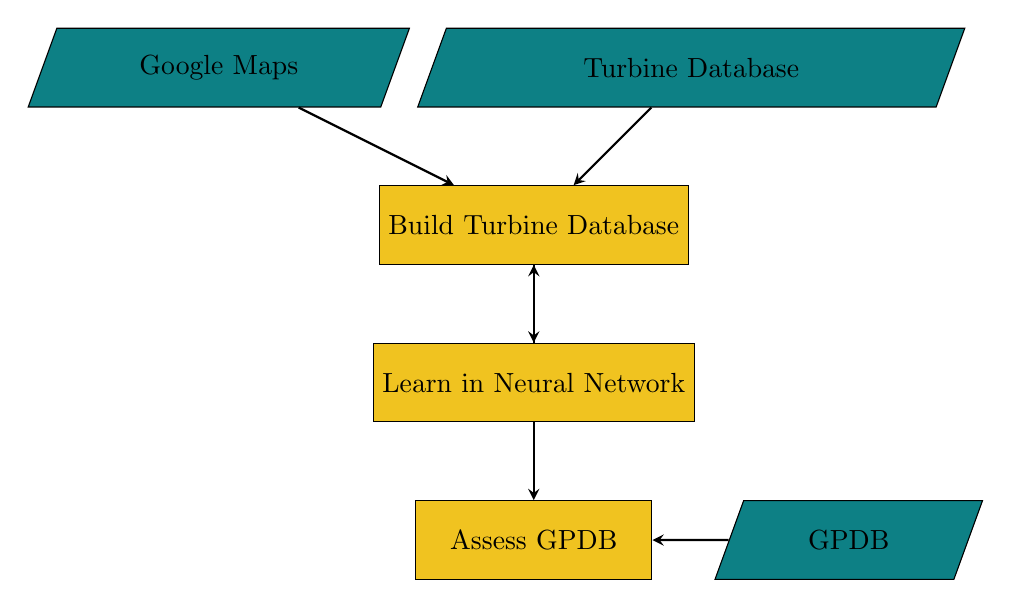
\begin{tikzpicture}[node distance=2cm]

%\node (Start) [startstop] {Start};

\node (in1) [io] {Google Maps};
\node (in2) [io, right of=in1, xshift=4cm] {Turbine Database};

\node (pro1) [process, below of=in1, xshift=4cm] {Build Turbine Database};


\node (pro2) [process, below of=pro1] {Learn in Neural Network};
\node (pro3) [process, below of=pro2] {Assess GPDB};
\node (in3)  [io, right of=pro3, xshift=2cm] {GPDB};


\draw [arrow] (in1) -- (pro1);
\draw [arrow] (in2) -- (pro1);

\draw [arrow] (pro1) -- (pro2);
\draw [arrow] (pro2) -- (pro1);
\draw [arrow] (pro2) -- (pro3);
\draw [arrow] (in3) -- (pro3);

\end{tikzpicture}

\end{frame}


\begin{frame}
\frametitle{Software}

\begin{itemize}
 \item Downloading of data from google maps: R (RGdal, tidyverse, raster)
 \item Machine Learning: Python (keras, scikit-image, gdal)
 \item Mixing R and Python: not a brilliant idea. Just lazy.
 
 
\end{itemize}

\end{frame}



\begin{frame}
\frametitle{Create Sample Database}
\framesubtitle{Manual quality control}

\center{
Positives
}

\begin{table}[ht]
\centering
\begin{tabular}{cccc}
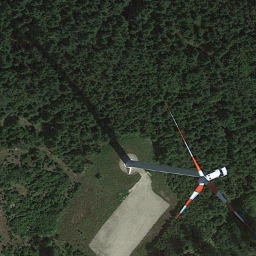
\includegraphics[width=0.2\linewidth]{../figures/wt_at_1.png}&
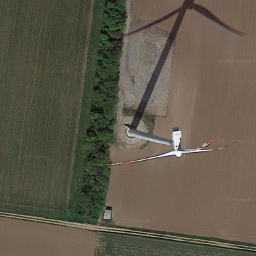
\includegraphics[width=0.2\linewidth]{../figures/wt_at_2.png}&
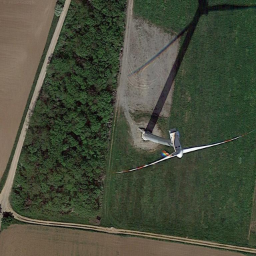
\includegraphics[width=0.2\linewidth]{../figures/wt_at_3.png}&
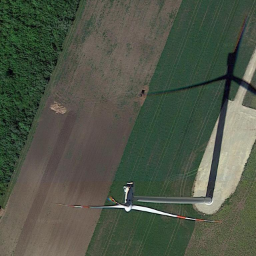
\includegraphics[width=0.2\linewidth]{../figures/wt_at_4.png}\\
\end{tabular}
\end{table}

\begin{center}
Negatives
\end{center}

\begin{table}[ht]
\centering
\begin{tabular}{cccc}
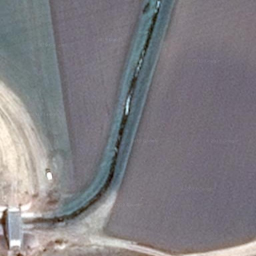
\includegraphics[width=0.2\linewidth]{../figures/no_wt_at_1.png}&
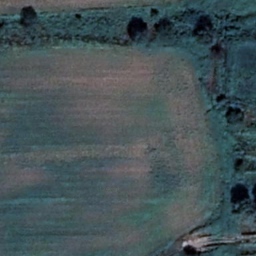
\includegraphics[width=0.2\linewidth]{../figures/no_wt_at_2.png}&
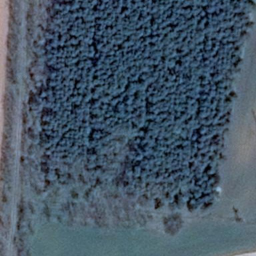
\includegraphics[width=0.2\linewidth]{../figures/no_wt_at_3.png}&
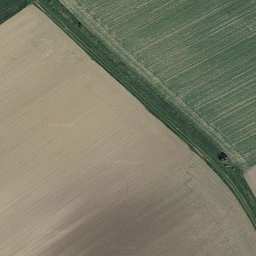
\includegraphics[width=0.2\linewidth]{../figures/no_wt_at_4.png}\\
\end{tabular}
\end{table}






\end{frame}


\begin{frame}
\frametitle{Learn with Convolutional layers}

\begin{center}
	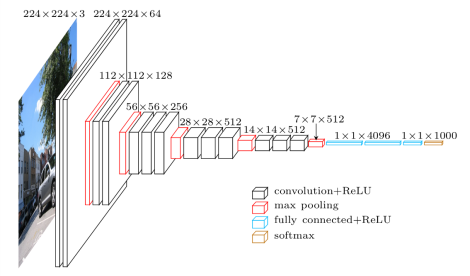
\includegraphics[width=0.8\linewidth]{../figures/vgg16.png}
\end{center}

\end{frame}

\begin{frame}
\frametitle{Layered feature learning}

\begin{figure}
	\centering
	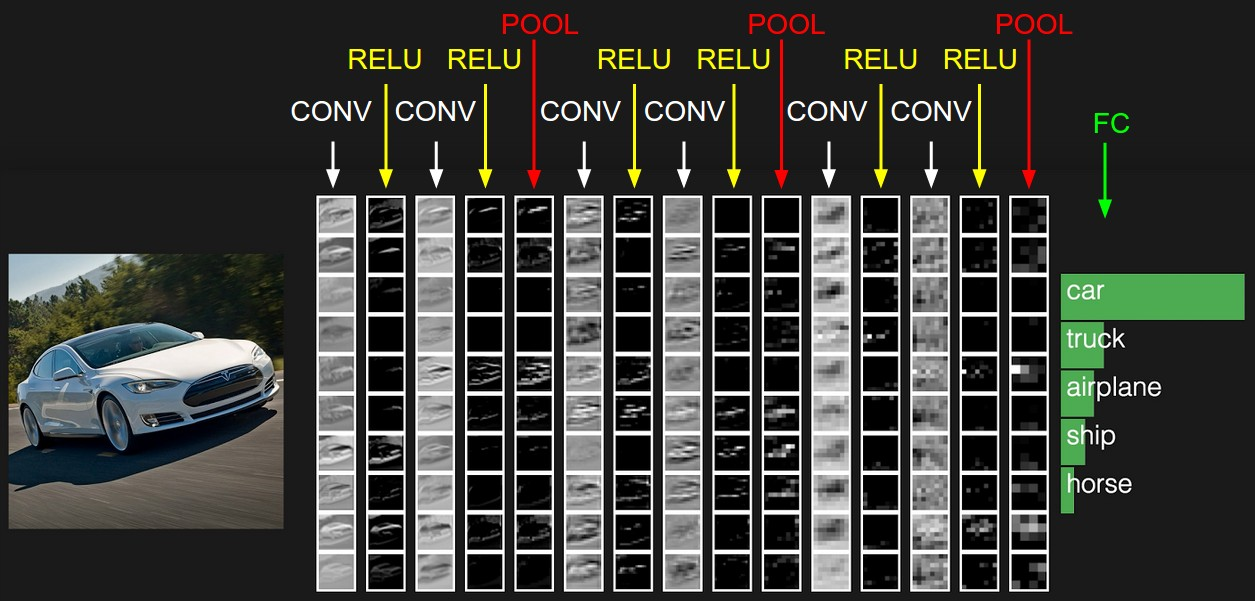
\includegraphics[width=0.8\linewidth]{../figures/convnet.jpeg}
	\caption{Taken from \href{http://cs231n.github.io/convolutional-networks/}{here}}
\end{figure}
\end{frame}

\begin{frame}
\frametitle{\href{https://ujjwalkarn.me/2016/08/11/intuitive-explanation-convnets/}{Terminology}}
\begin{itemize}
	\item Convolution operation
	\item Filter
	\item Depth
	\item Stride
	\item Zero padding (wide and narrow convolution)
\end{itemize}
\end{frame}

\begin{frame}
\frametitle{Pooling}
\begin{itemize}
	\item Makes input representations (feature dimension) smaller and more manageable
	\item Reduces the number of parameters and computations in the network controlling overfitting
	\item Makes the network invariant to small transformations, distortions and translations in the input image
	\item Helps us arriving at an almost scale invariant representation of our image (the exact term is “equivariant”)
	\item taken from \href{https://ujjwalkarn.me/2016/08/11/intuitive-explanation-convnets/}{here}
	
\end{itemize}


\end{frame}

\begin{frame}
\frametitle{Some hints}
\begin{itemize}
	\item Compile high quality training set
	\item Do not overfit!	
	\item Use pretrained networks to speed up learning process. Keras models can be found \href{https://keras.io/applications/}{here}
	\item Unfreeze last layers to learn your specific task, fixing the lower layers which extract basic features
	
\end{itemize}
\end{frame}

\begin{frame}
\frametitle{Results Learning}
\framesubtitle{Quality Measures}
\begin{centering}
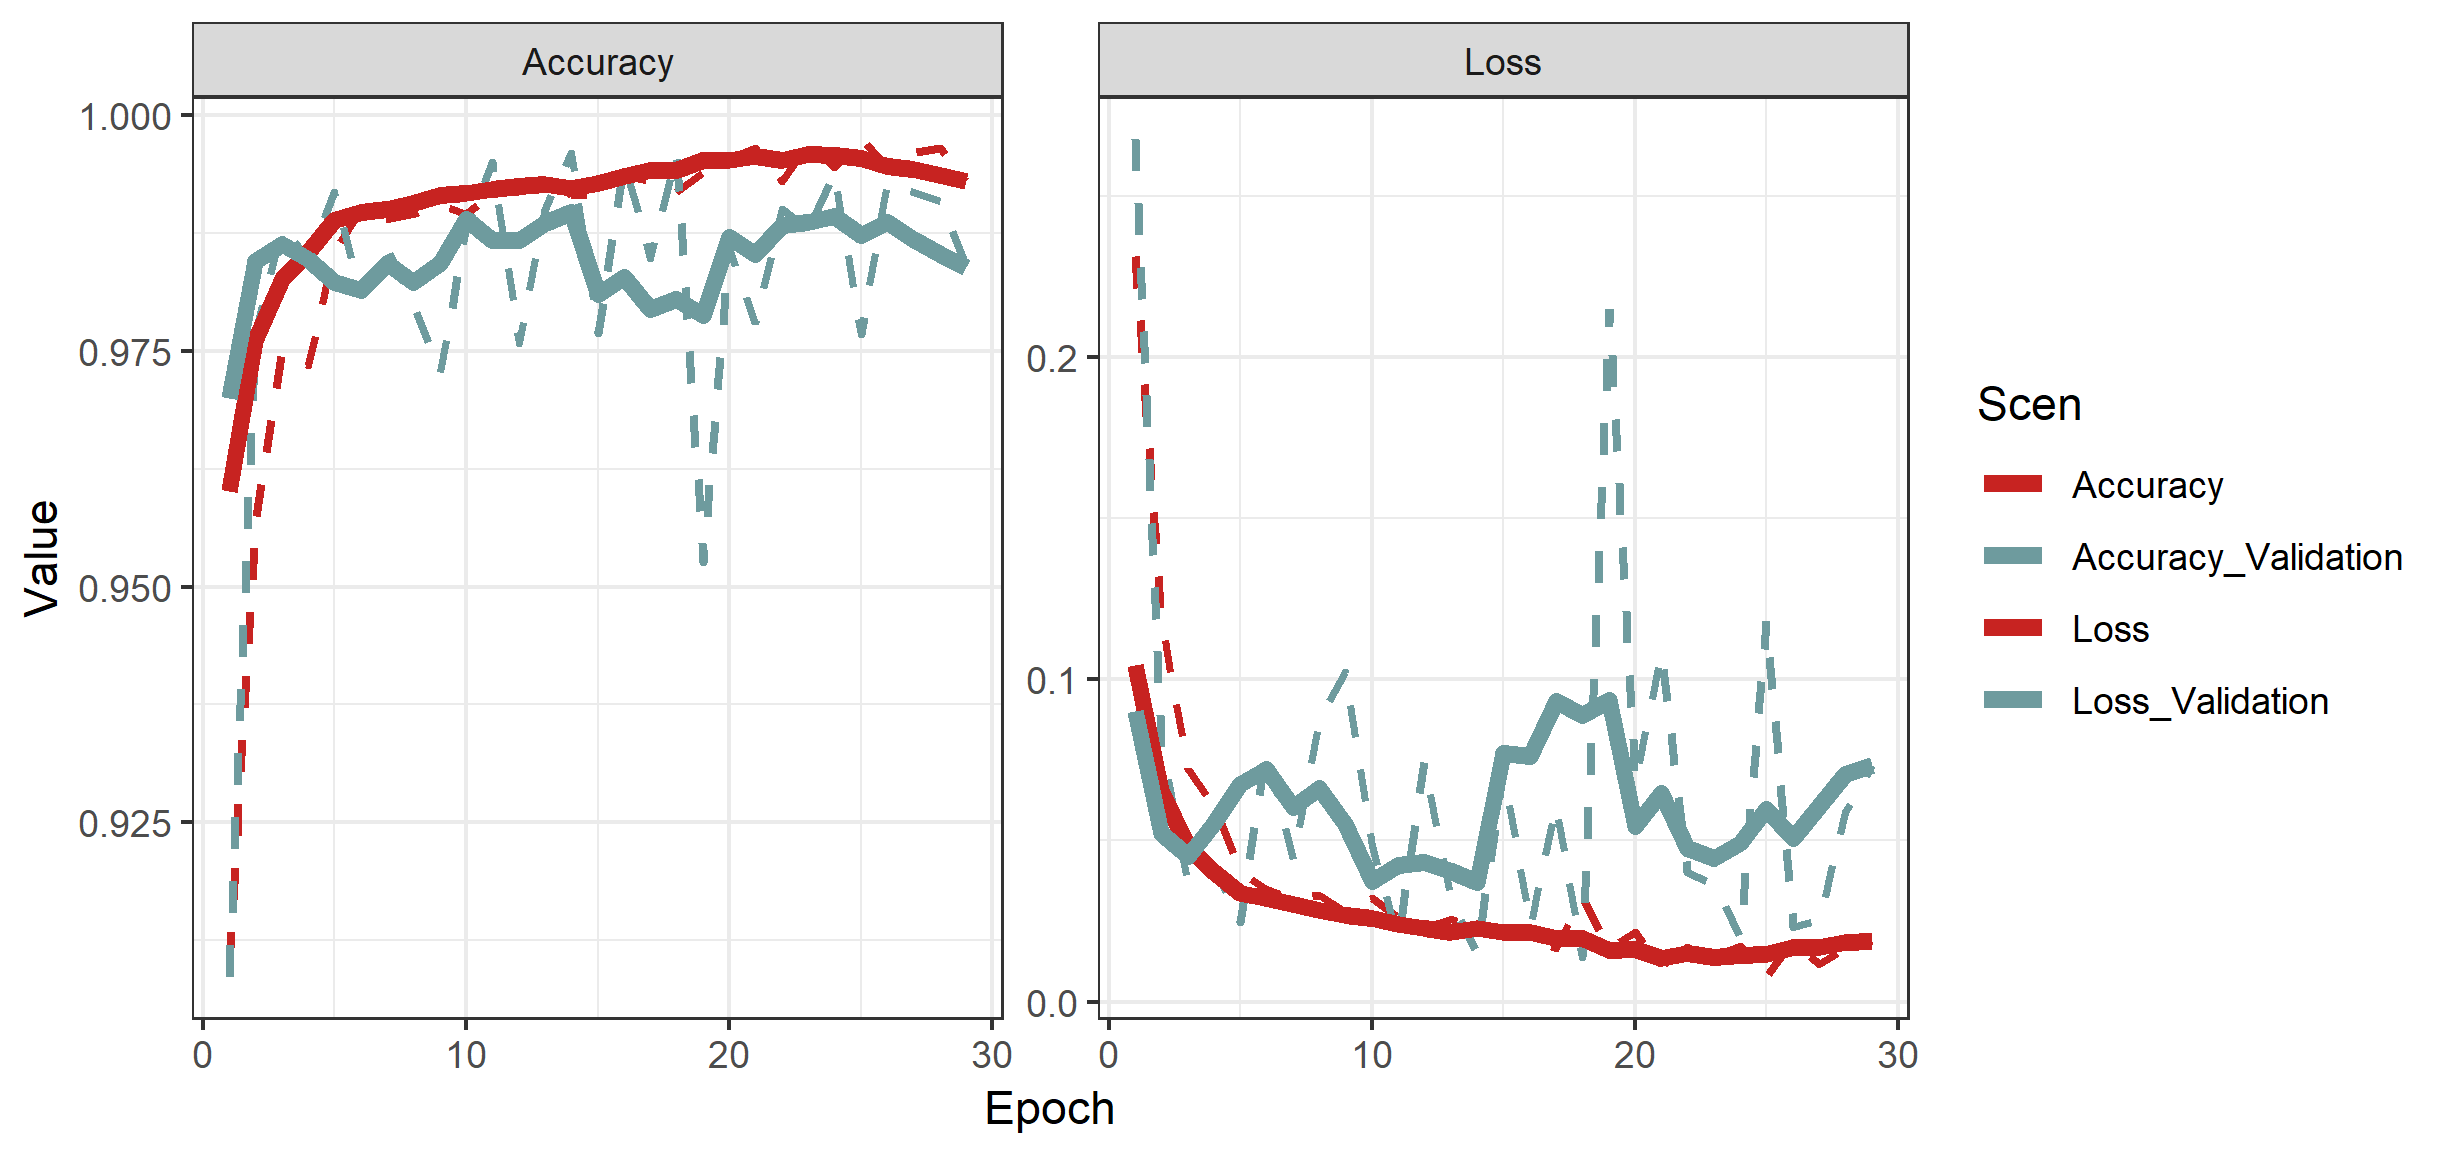
\includegraphics[width=\linewidth]{../figures/accuracy_loss.png}
\end{centering}


\begin{centering}
\begin{table}[ht]
\centering
\begin{tabular}{cc}

\tiny{
$Accuracy=\frac{Number\ of\ Correct\ Predictions}{Number\ of\ Total\ Predictions}$
} 

&
\tiny{
$Loss=-1\frac{1}{N}\sum_{i=1}{N}y_ilog(p(y_i))+(1-y_i)log(1-p(y_i))$
}

\\


\end{tabular}
\end{table}
\end{centering}

\end{frame}



\begin{frame}
\frametitle{Results Learning}
\framesubtitle{Class Activation Map}

% READ THIS: https://jacobgil.github.io/deeplearning/class-activation-maps
% makes sense for the handmade network and should make sense for the vgg16 one.

\begin{centering}

\begin{table}[ht]
\centering
\begin{tabular}{cc}

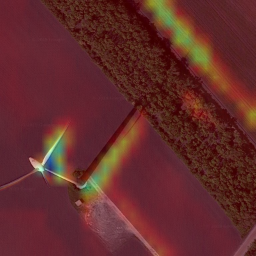
\includegraphics[width=0.4\linewidth]{../figures/heatmap_turbine.png}&
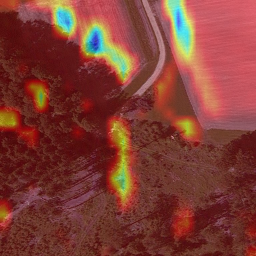
\includegraphics[width=0.4\linewidth]{../figures/heatmap_no_turbine.png}\\
\small {Probability of being wind turbine 0.999} &
\small {Probability of being wind turbine 0.001} \\

\end{tabular}
\end{table}


\end{centering}


\end{frame}




\begin{frame}
\frametitle{Searching wind turbines}
\framesubtitle{Create grid and check image by image}

\center{

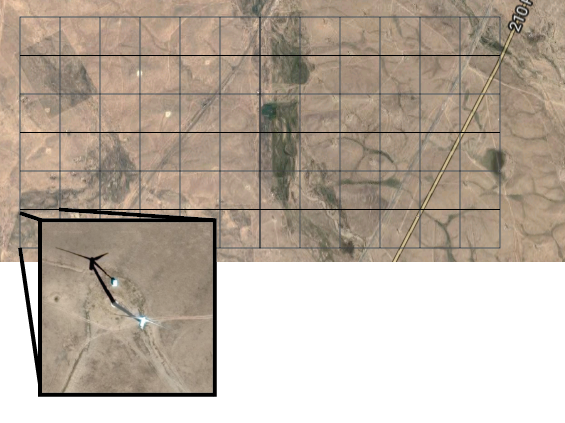
\includegraphics[width=0.8\linewidth]{../figures/grid_search.png}
}

\end{frame}



\begin{frame}
\frametitle{Application}
\framesubtitle{Chinese and French Wind Parks}
\textbf{China}: 28 parks assessed. Found 266 turbines. 83 wrongly classified (manual control). At 7 out of 28 park locations no turbine was found.\\

\textbf{France}: 10 parks assessed. Found 27 turbines. 15 wrongly classified (manual control). At 5 out of 10 park locations no turbine was found.

\end{frame}

\begin{frame}
\frametitle{Discussion}
\begin{itemize}
 \item Dates of satellite photos and dates of turbine installations unknown
 \item Shaky legal conditions
 \item Runtime prohibitive on desktop computers. For a full global check would need cluster computing with high bandwidth (but see shaky legal conditions...) 
 \item Classification has to be extended to be applicable to different world regions. Applying Austrian/Brazilian conditions to China/France does not work very well (i.e. classification errors).
\end{itemize}

\end{frame}




\begin{frame}
\frametitle{Conclusions}
\begin{itemize}
 \item Full validation of GPDB due to missing temporal information not fully possible. However, first assessments of accuracy possible.
 \item Current best commercial satellite data allows identification of single turbines with good accuracy by using machine learning approaches
 \item Research limited by Data availability. Public domain data is low resolution (i.e. Sentinel-2) or small spatial domain (free ortho-photos, like basemmap.at).
\end{itemize}

\end{frame}




{
\usebackgroundtemplate{
 \begin{picture}(320,315)
 \hspace{6.9cm}
   
\includegraphics[width=0.7\linewidth]{../figures/refuel_logo_with_text.png}
 \end{picture}
 }


\begin{frame}
\frametitle{Thank you!}
\begin{block}{
 For updates on the project, check \textbf{refuel.world}\\
 For source-code, check \textbf{github.com/joph/MachineLearningCourse}\\
 
		mail: johannes.schmidt@boku.ac.at\\

}
\end{block}

\vspace{2.5 cm}


\end{frame}

}


\end{document} 